\documentclass[tikz,border=0pt]{standalone}
\usepackage{fontspec,xeCJK,graphicx}
\setmainfont{Times New Roman}
\setCJKmainfont{SimSun}
\begin{document}
\begin{tikzpicture}[x=1cm,y=1cm,every node/.style={inner sep=0pt,font=\fontsize{9bp}{11bp}\selectfont}]
\path[use as bounding box] (0,0) rectangle (17.4,9.1);
\node[anchor=south west] at (0,1.8) {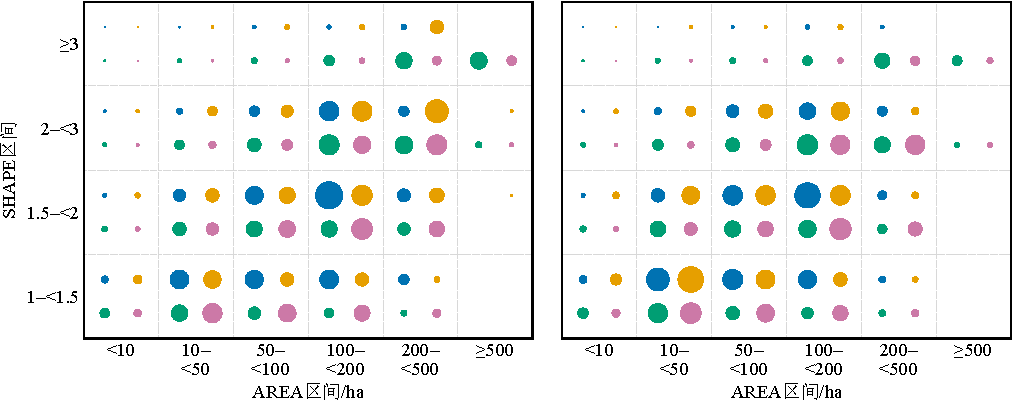
\includegraphics{frames.pdf}};
\node at (5.3,1.80) {（a）玉米};
\node at (13.4,1.80) {（b）大豆};
\node[anchor=west] at (1.4,1.30) {站点};
\definecolor{siteA}{HTML}{0072B2}
\fill[siteA] (2.5000,1.30) circle[radius=0.09cm];
\node[anchor=west] at (2.6700,1.30) {A};
\definecolor{siteB}{HTML}{E69F00}
\fill[siteB] (3.5000,1.30) circle[radius=0.09cm];
\node[anchor=west] at (3.6700,1.30) {B};
\definecolor{siteC}{HTML}{009E73}
\fill[siteC] (4.5000,1.30) circle[radius=0.09cm];
\node[anchor=west] at (4.6700,1.30) {C};
\definecolor{siteD}{HTML}{CC79A7}
\fill[siteD] (5.5000,1.30) circle[radius=0.09cm];
\node[anchor=west] at (5.6700,1.30) {D};
\node[anchor=west] at (7.0,1.30) {作物面积占比};
\definecolor{bubblegray}{HTML}{777777}
\fill[bubblegray] (9.650000,1.30) circle[radius=0.048570216690cm];
\node[anchor=west] at (9.828570,1.30) {1\%};
\fill[bubblegray] (11.250000,1.30) circle[radius=0.108606306201cm];
\node[anchor=west] at (11.488606,1.30) {5\%};
\fill[bubblegray] (13.050000,1.30) circle[radius=0.217212612401cm];
\node[anchor=west] at (13.397213,1.30) {20\%};
\node[anchor=west] at (0.1,0.82) {每格A左上、B右上、C左下、D右下；位置偏移仅用于区分站点，不表示档内数值差异。};
\node[anchor=west] at (0.1,0.39) {气泡圆面积表示该站该作物的面积占比；分档仅供探索，气泡代表档内汇总，不代表单个斑块。};
\end{tikzpicture}
\end{document}
